\documentclass[../thesis.tex]{subfiles}

\begin{document}

\section{Current Methods for Localizing Objects Using Contact Sensors}

Before performing operations on parts for manufacturing, it is crucial that the position and orientation of that part are known to within some tolerance.
While there are many methods of localizing a part, this work uses a touch probe to actively gain information through measurements on the part surface.
Though it is possible to ignore uncertainty in some tasks, the this work explicitly reasons over the belief distribution of the part's state to address more challening tasks.
One approach, the particle filter, maintains this distribution through a finite set of samples.
A second approach, the Kalman filter, maintains an analytic expression for the belief distribution.
Both approaches require adaptations for use in contact localization.

%% This localization can be provided by fixturing, human vision, computer vision, ranged sensors, touch probes, and other methods.
%% In some situations the fixturing such as vices, jigs, and guides provide suffient localization, and active sensing is unnecesary.
%% But in other situations dedicated sensors provide measurements used to localize the part.

%% Touch probes are a staple in machine shops for precicely localizing parts.
%% In simple cases fixturing localizes many of the degrees of freedom of a part, leaving perhaps only a single dimension with uncertainty that the probe must resolve.
%% While there is uncertainty in every measurement, it is not always necessary to model that uncertainty, and in some cases simply proceeding 



\subsection{Particle Filters}
Particle filters, touch measurements, and maximal information gain measurement selection have all been used in localization tasks. 
Since their introduction particle filters have been popular due to their ease of implementation and ability to model complex distributions, process models, and measurement models \cite{Thrun2000a}. 
However, for a measurement with low uncertainty there exists only a thin manifold of states consistent with that measurement, yielding a low probability of any particle existing on that manifold, leading to particle starvation \cite{Thrun2000}.
Handling particle starvation is described in detail in Chapter \ref{sec:pfilterProblems}.

To address particle starvation, Koval et al. introduced the Manifold Particle Filter, using different sampling methods depending on the volume of the space consistent with a measurement \cite{Koval2011, Koval2013}. 
This allows a quick update of the belief when the contact sensor is not in contact with the part, and only requires addressing the harder thin manifold update problem when contact is made. 
Koval used multiple methods when updating from measurements when on this thin manifold, and shows that rejection sampling requires the fewest restrictions on prior knowledge of the environment, but naive rejection sampling is time consuming.
His efficient methods require direct sampling from the contact manifold, which is not feasible for a complex part.

Petrovskaya et al. focused on global localization of objects via touch \cite{Petrovskaya2011} and introduced the Series Scaling algorithm to overcome particle starvation. 
The Series Scaling algorithm adaptively alters the particle density depending on the complexity of the posterior. 
Multiple passes through the measurement data are used and the precision of the modeled belief is scaled from low to high, avoiding unnecessarily precise estimates in exceedingly unlikely regions of belief space. 
This is complementary to our approach, and implementing multiple passes on our methods could lead to a faster update process.

Much of the recent work on touch measurements uses a robotic hand with contact sensors. In these works evaluation of both actual and simulated measurements required collision checking between two meshes which is computationally expensive. 


Hebert et al. use geometric (CAD) models of objects such as screwdrivers and door handles as well as the geometric model of their robotic arm to autonomously choose touch actions that localize objects sufficiently to perform everyday tasks, such as grasping and opening doors. 
Their algorithm greedily selects the next best touch action from a list of candidate actions to maximize information gain \cite{Hebert2013}.


Javdani et al. shows that selecting the next touch to maximize information gain is submodular under assumptions of a static object and an action cost independent of object and robot state, explaining the effectiveness of the greedy approach \cite{Javdani2013}. 
This provides a sound theoretical basis for our approach.
Javdani demonstrates the computation of information gain is time consuming and proposes an alternative method of hypothesis pruning. 
Our formulation computes the expected information gain about two orders of magnitude faster, and thus we are able to evaluate many more potential measurement actions and model the belief using more particles.



Recently, there have been a variety of approaches that allow robots to localize objects solely with contact sensors. Different contact sensors have been explored and developed, including basic binary sensors, 6-axis force and torque sensors \cite{del2012control}, soft tactile sensor arrays \cite{hammond2012soft}, and bio-inspired fingertips \cite{fishel2012sensing}. Localization with laser sensors has also been used in the high-precision CNC localization, where a 3D point cloud is acquired in order to estimate the transformation between the actual and planned pose \cite{rajaraman2013automated}.
The localization approach presented here can be generalized to these sensors which can distinguish between contact and free-of-contact states.



\subsection{Kalman Filters}
Alternative approaches to modeling touch localization adapt a Kalman Filter to model the belief distribution \cite{Choukroun2006}\cite{Srivatsan}.
A Kalman filter requires a Gaussian belief of the estimated state, which is inaccurate in touch localization. 
For example, multi-modal distributions appear when it is ambiguous whether a close edge or far edge was touched. %% Non-Gaussian distributions also occur even when the touched edge is known.

A Kalman filter also requires a linear measurement models, which does not exist for touch localization, so this too must be approximated.
The Extended Kalman Filter performs first-order linear approximations of the measurement model, but this diverges for pose estimation with large initial error \cite{Choukroun2006}.
The Unscented Kalman Filter approximates the measurement model through evaluation at many ``sigma'' points chosen by tuning parameters.
As the pose likelihood given a measurement varies by many orders of magnitude in different dimensions, these parameters are sensitive and unreliable.
Srivatsan et al. constructs a linear measurement model using two measurements and assuming the correspondence between the probe tip and the touched point on the object \cite{Srivatsan}.
This allows direct use of a Kalman filter with a true measurement model.
However, the true correspondence is unknown, and must be approximated, for example through Iterative Closest Point (ICP) methods.

The approach in this thesis uses a Gaussian kernel applied to set of discrete particles, similar to a mixture of Gaussians model \cite{Thrun2000}, allowing multimodal beliefs.
Neither a local linear approximation to the measurement model, nor correspondence between the probe tip and touched object point are required.


%% Particle filters have been widely used and developed since their introduction. 
%% Unlike some other Bayesian estimation approaches such as Kalman filters \cite{kalman1960new}, extended Kalman filters \cite{kalman1961new} and unscented Kalman filters \cite{julier1997new}, particle filters can easily model non-Gaussian and multi-modal probability distribution. 
%% For touch localization, contact sensors yield a highly non-linear measurement model, and the belief can frequently become multi-modal when multiple configurations are all consistent with the measurement. 
%% These properties make particle filter a popular approach for touch localization tasks. 

%% However, particle filters will experience \textit{particle starvation} for measurements with very low uncertainty and objects with a high dimensional configuration space \cite{Thrun2000}. 
%% Koval introduced the Manifold Particle Filter to address this issue by implementing different sampling and weighting strategies compared to the traditional particle filters \cite{Koval2011}\cite{ Koval2013}. 
%% Instead of sampling particles from the process model and weighting them based on the observation, samples are directly drawn from the contact manifold, given the observation. 
%% This provides a fast and robust solution for objects with simple shapes. 
%% For complex object geometries, as in this case, direct, efficient sampling from the contact manifold becomes difficult.

%% Petrovskaya tackles particle starvation during touch localization by combined Monte Carlo approaches with annealing as a smoothing technique \cite{Petrovskaya2011}. 
%% She introduced Scaling Series algorithms for 6-DOF global tactile localization in both full-constrained and under-constrained scenarios to overcome particle starvation by adjusting particle density depending on the complexity of the posterior. 
%% Multiple iterations through the measurement data are used and the precision of the belief is scaled from low to high in order to avoid unnecessarily precise estimates in unlikely regions of belief space. 


%% All of the work mentioned so far assumes the prior information of the object geometry matches the real piece perfectly. 
%% Hebert et al. \cite{Hebert2013} solve a touch localization problem using a Bayes filter where an object may have additional unknown parameters describing the shape, such as a screw driver with an unknown length handle.
%% Measurement actions are selected using joint information gain over the object's pose and these internal parameters.
%% To the best of our knowledge, our proposed method is the first one that handles localization problems for object with coupled datums.





%%%%%%%%%%%%%%%%%%%%%%%%%%%%%%%%%%%%%%%%%%%%%%%%%%%%%%%%%%%%%%%%%%%%%%%%%%%%%%%%%%%%%%%
\section{Contacts in Planning}

Higher level tasks involve frequent making and breaking of contacts:
walking requires footstep placement, manufacturing involves part handling, and household tasks need object manipulation.
The wide variety of sub-problems lead to different approaches to robotic reasoning and execution of actions with contacts.
In some tasks the the robot must decide between a known set of fixed contact locations, while in other tasks the contact space is continuous.
Contacts may be a necessity or they may be optional.
%% Advancements in robots planning for contacts have occured 
%% There are many approaches

In many path planning problems, any contact with the environment is considered a collision and thus valid paths have no interaction with the environment.
However environmental contacts can reduce joint torques, damp vibrations, and stabilize an arm.
Despite these benefits contacts are usually avoided because they bring algorithmic complexity during the planning stage and physical danger to the robot and environment if executed improperly.
The increased planning complexity is due to the contact configurations being a measure-zero manifold in the robot configuration space, rendering naive planning in configuration space ineffective. 


\subsection{Bracing, Climbing, and Walking}
The benefits of bracing have been studied since the 1990s.
Lew and Book proposed bracing a micro/macro manipulator with small precise arm mounted on the end of a long coarse arm and demonstrated bracing of the macro arm against multiple locations of the environment can damp vibration caused by the micro arm \cite{Book1994} \cite{Lew1993}.
Hollis and Hammer explored a similar micro/macro robot design and demonstrated $1 \mu m$ accuracy, well over an order of magnitude improvement compared to their unbraced manipulator \cite{Hollis1992}.
Both of these works did not address the planning problem as both contact locations and robot trajectories were manually specified.


Given a sequence of contact modes for each link, Greenfield computed joint torques to produce desired dynamic behavior and applied this to a climbing snake robot \cite{Greenfield2005}.
Bretl et al. \cite{Bretl2006} developed algorithms for climbing robots that first select contact locations then create collision free trajectories for the robot's limbs between these contact locations.

The recent DARPA Robotics Challenge showcased state of the art walking robots.
Rather than solving for a trajectory and contact locations simultaneously some approaches have separated these two problems.
The dominant planning architectures hierarchically separated stages of contact planning.
Highest, and slowest, in the hierarchy a planner decides the path for a simplified model of the robot through the workspace using heuristic costs.
Lower down in the hierarchy, a footstep planner determines the contact locations for feet to best achieve the higher level trajectory.
Still further down, another planner determines joint trajectories to move the feet into the requested footstep locations while maintaining stability  \cite{Deits2015} \cite{Atkeson2015}.
Tonneau et al. \cite{Tonneau} approaches from the opposite direction and first generates a trajectory then considers a discrete set of contacts close to that trajectory.



\subsection{Sample Based Planning} \label{sec:related:RRT}
Sampling based planners probabilistically probe the configuration space searching for feasible paths.
The valid configuration space is never explicitly represented, and all that is needed is a function that determines whether a specific configuration is valid.
The Rapidly-exploring Random Tree (RRT) is a sampling based planner which build trees of valid trajectories (edges) between points in configuration space (nodes).
To grow these graphs a new point in configuration space is sampled, and the closest point on the existing tree is extended towards this sampled point, as shown in Algorithm \ref{alg:RRT} \cite{LaValle1998}.

\begin{algorithm}
  \caption{$T=(V,E) \leftarrow$ RRT$(x_{start})$} \label{alg:RRT}
  \begin{algorithmic}[1]
    \State $T \leftarrow$ InitTree( $x_{start}$ )
    \While {GoalNotReached($T, X_{goal}$)}
    \State $x_{sample} \in X \leftarrow$ Sample()
    \State $x_{nearest} \leftarrow $ Nearest($T, x_{sample}$)
    \State T $\leftarrow Extend(x_{nearest}, x_{sample}, T)$
    \EndWhile
  \end{algorithmic}
\end{algorithm}

In the most basic implementation, the Extend function constructs a linearly trajectory in configuration space from $x_{nearest}$ towards $x_{sample}$, and terminates the extension either when $x_{sample}$ is reached or the trajectory enters an invalid region \cite{LaValle1998}.
This extension step requires augmentation to be useful in planning with contacts.
Sampling based planners will never sample directly on the measure-zero contact manifold, and linearly extending a contact configuration to a new sampled point will immediately leave the contact manifold, immediately entering an invalid region in configuration space, producing no progress.

\begin{figure}
  \centering
  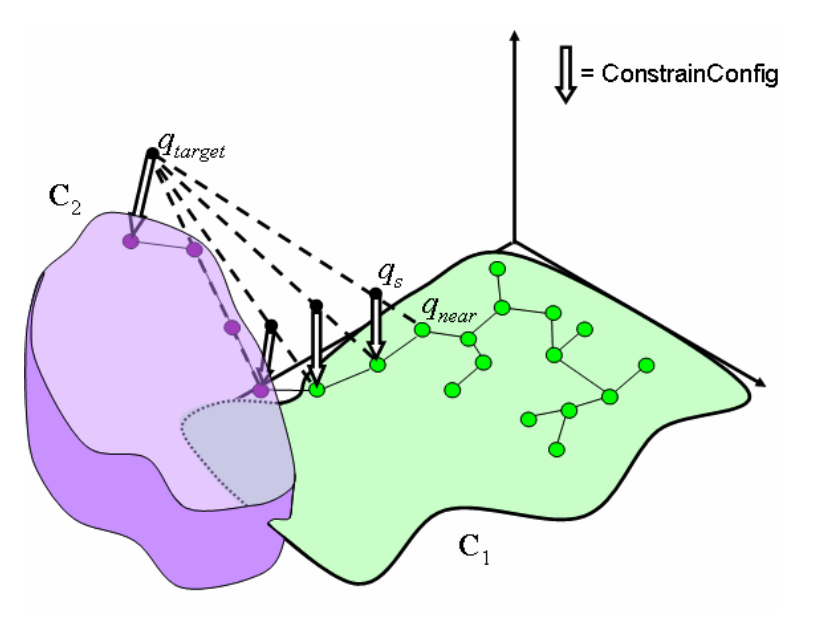
\includegraphics[width=.5\linewidth]{./RelatedWork/CBiRRT.png}
  \caption{Constrained Bidirectional Rapidly Exploring Random Tree (CBiRRT) extending the tree onto a measure-zero valid manifold in configuration space}
  \label{fig:CiBRRT}
\end{figure}


Berenson developed a variation of an RRT planner capable of handling measure-zero manifolds by projecting invalid path extensions onto the valid configuration space \cite{Berenson2009a}.
The Constrained Bi-directional RRT (CBiRRT) performs a linear extension from $x_{nearest}$ towards $x_{sample}$ as before, producing an intermediate point $x_s$.
However if $x_s$ is an invalid configuration, a projection function is used to potentially create a valid configuration.
\begin{align}
  x_s^{new} \leftarrow Projection(x_s)
\end{align}
If $x_s^{new}$ is valid and is making progress toward $x_{sample}$, the extension algorithm continues.
If either the $Projection$ function failed to produce a valid configuration, or the extension toward $x_s^{new}$ moves the trajectory further from $x_{sample}$ then extension is terminated and the RRT algorithm continues with a new randomly sampled point.
In CBiRRT the method of projection must be provided by the user, and it is not obvious how to construct a productive projection function for an arm where multiple contacts are allowed. 
This thesis uses a sampling based planner that is able to traverse thin manifolds by using a cost function, instead of a projection function, to guide the extension.



\subsection{Trajectory Optimization}
In contrast to sampling based planners, trajectory optimization addresses the path planning problem by incrementally improving an initial trajectory.
Trajectory optimization uses a cost function to assign a cost to every trajectory, and an initial trajectory is repeatedly adjusted to reduce this cost.
While a large class of work focuses on trajectory optimization with unknown dynamics, in this thesis it is assumed the dynamics are known, and the guiding approach is to assume the dynamics are locally linear and perform updates to the parameters of the trajectory based on the gradient of the cost function.
This approach will converge to local, but not necessarily global, minimal cost trajectories.
Contact forces present an initial challenge, as the assumption of locally linear dynamics no longer holds.

Deits et al. handles the foot placement contacts for walking robots through mixed-integer optimization \cite{Deits2015}.
In a path for a walking robot there are an integer number of footstep placements, but the trajectories of the feet and robot are continuous.
One approach is to fix the number of footsteps and run a purely continuous optimization over the trajectories.
This continuous optimization is then repeated for each integer number of footsteps considered plausible.
To reduce the number of optimization, their approach assigns a cost to each footstep allowing for faster pruning.
This approach works because the integer parameter is relatively simple, i.e. once the right foot steps the only next contact to consider is the left foot.


Both Posa et al. \cite{Posa2013} and Mordatch et al. \cite{Mordatch2012}  handle the discontinuous contacts by smoothing.
Both formulations assume a given set of locations on the robot are allowed to make contact with the given environment.
Both works write the cost of a trajectory as a function of both joint torques and contact forces, thus the contact forces are a slack variable, and treated as parameters of the trajectory.
Of course, in reality, a robot cannot choose the contact force applied, as the force is generated by electron repulsion as a function of the distance between the environment and the robot.
However, this inaccurate physics model smooths the cost function and allows the robot to discover the benefits of contacts.
Additional constraints are imposed to ensure the final trajectory is physically feasible.


Posa et al. \cite{Posa2013} is primarily concerned with large impact forces, and writes the problem as a constrained optimization.
At each iteration the optimizer alters both the joint torques and the desired contact forces to improve the cost.
However this optimization problem has a set of complementarity constraints which enforce that each section of the robot is either in contact and can receive a contact force, or is not in contact.

Mordatch et al. \cite{Mordatch2012} designed an approach called contact invariant optimization, where a cost continuously models both the benefit and cost of adding contacts and is able to produce trajectories which add and break contacts.
This formulates the problem as a purely unconstrained optimization, with all physical constraints being added to the cost function.
The parameters of this cost function are both the joint torques and a set of continuous ``contact'' slack variables, one for each section of the robot that is allowed to make contact.
For each section, the contact variable can be intuitively be thought of as trade off between the benefits and the challenges of making contact with the environment.
Increasing the contact variable increases the cost as a function of the distance between the robot section and the environment.
Increasing the contact variable decreases the cost as it allows contact forces to compensate for joint torques.
Of course in reality there is no partial contact, as if a section of a robot is some distance away from the environment, no contact force is applied.
However this formulation of force at a distance makes the benefit of adding a contact visible to the gradient of the cost function.
To ensure the final trajectory is feasible, the cost of physically infeasible partial contacts is increased dramatically towards the end of the optimization. 

This thesis uses a similar approach to Mordatch's contact invariant optimization to construct an unrealistic but useful dynamics model.
Experiments demonstrate these methods on physical robots.


\end{document}
